%%% Local Variables:
%%% mode: latex
%%% TeX-master: t
%%% End:

\chapter{基于光敏高分子的三维光子晶体图案化的研究}
\label{ch:photoactive}

\section{引言}
第~\ref{ch:maleimide}章中展示了基于化学反应的光子晶体材料在生物传感及其相关方面的应用,证明了基于化学反应的光子晶体材料的巨大应用前景。但通过一次成型制备的光子晶体材料仅能呈现单一的结构色,且化学成分呈现各向同性。
对光子晶体的图案化因此具有重要的意义。一方面,图案化光子晶体的制备使得光子晶体材料摆脱了单一的结构色外观而具有实际应用价值;另一方面,基于化学修饰的图案化光子晶体具有二维的化学结构复杂性,这种区域特异性的化学组成与光子晶体的光学性质及反蛋白石结构的内部孔道相结合,有助于形成功能丰富的新型材料。

在~\ref{sec:multiscale-phc}节对目前光子晶体图案化方法的概述中我们可以看到,大部分的光子晶体图案化方法的着眼点在对正模板或复合结构的光子晶体进行修饰,而对反蛋白石结构的光子晶体的图案化修饰所见报道较少。
一方面,反蛋白石结构自身的完整性使物理刻蚀法或拓扑法等难以实现;另一方面,反蛋白石内部的孔道结构造成的扩散也使得液体存在扩散,限制了压印或液滴法的应用。
尽管无法在反蛋白石一次成型的过程中便对其进行图案化,我们仍能够采用选择性的后修饰法来赋予光子晶体不同区域差异性的化学组成。
本章中便提出一种基于选择性化学修饰法来对三维光子晶体进行图案化修饰的方法。
首先,组成反蛋白石光子晶体的高分子具有可以选择性脱保护的官能团,在一定的条件下脱去活性官能团的保护基。由于化学反应的选择性,当后修饰的化合物与光子晶体接触时,只有活性暴露了活性官能团的部分才能够参与化学反应;而未脱保护的官能团则保持原样,并可以在下一轮的修饰中被继续脱保护-修饰。
受惠于化学反应的特异性,这种修饰方法能够避免液体在反蛋白石孔道中扩散造成的影响,因为只有选择性脱保护的官能团能够参与反应。同时,在整体操作过程中,反蛋白石光子晶体的内部结构能够得到很好的保留,避免了物理修饰法对结构的破坏。

理论上,任何具有可控脱保护的保护基均可以作为这里的活性基团保护基,但考虑在平面上的图案化操作及反应条件的温和性,这里采用紫外光照射的方法来实现脱保护的目的。
由于光的直线传播,因此可以使用光掩膜法来实现较精细的图案调控;同时,选用合适的紫外光脱保护条件能够实现在温和条件下的脱保护,减少加热脱保护(例如上一章中马来酰亚胺的脱保护)对光子晶体形貌及内部结构的影响。
这里我们选用2-硝基藜芦醇甲酸酯(NVOC)保护基来对聚合物中的氨基官能团进行保护\cite{Patchornik1970Photosensitive,Braun2003Novel}。
\begin{figure}[htbp]
  \centering
  
\includegraphics[width=\linewidth]{figures/ch4/NVOC-principle.png}
  \caption{NVOC保护基在紫外光条件下脱保护的原理示意图}
  \label{fig:NVOC-UV-principle}
\end{figure}

如图~\ref{fig:NVOC-UV-principle}所示,NVOC保护的氨基在360 nm左右的紫外光照射条件下经历自由基历程而释放出被保护的氨基基团,NVOC基团则转化为其对应的亚硝基产物而失去保护活性。NVOC保护基较早便在在氨基酸的氨基保护中具有一定的应用\cite{Barltrop1965883},但在液相反应中由于离去基团无法分离而具有较长的反应时间。而聚合物中的NVOC保护基由于离去基团能够被清洗等方法去除而具有很高的反应效率\cite{Cameron1991Photogeneration,Cui2012Phototunable},因此适用于这里的图案化修饰需求。在通过紫外脱保护后,暴露的氨基基团能够与较高活性的异氰酸酯化合物或活化羧酸酰胺化,从而实现对特定区域光子晶体的化学修饰。
其基本原理可见图~\ref{fig:photolabile-pattern-principle}。

\begin{figure}[htbp]
  \centering
  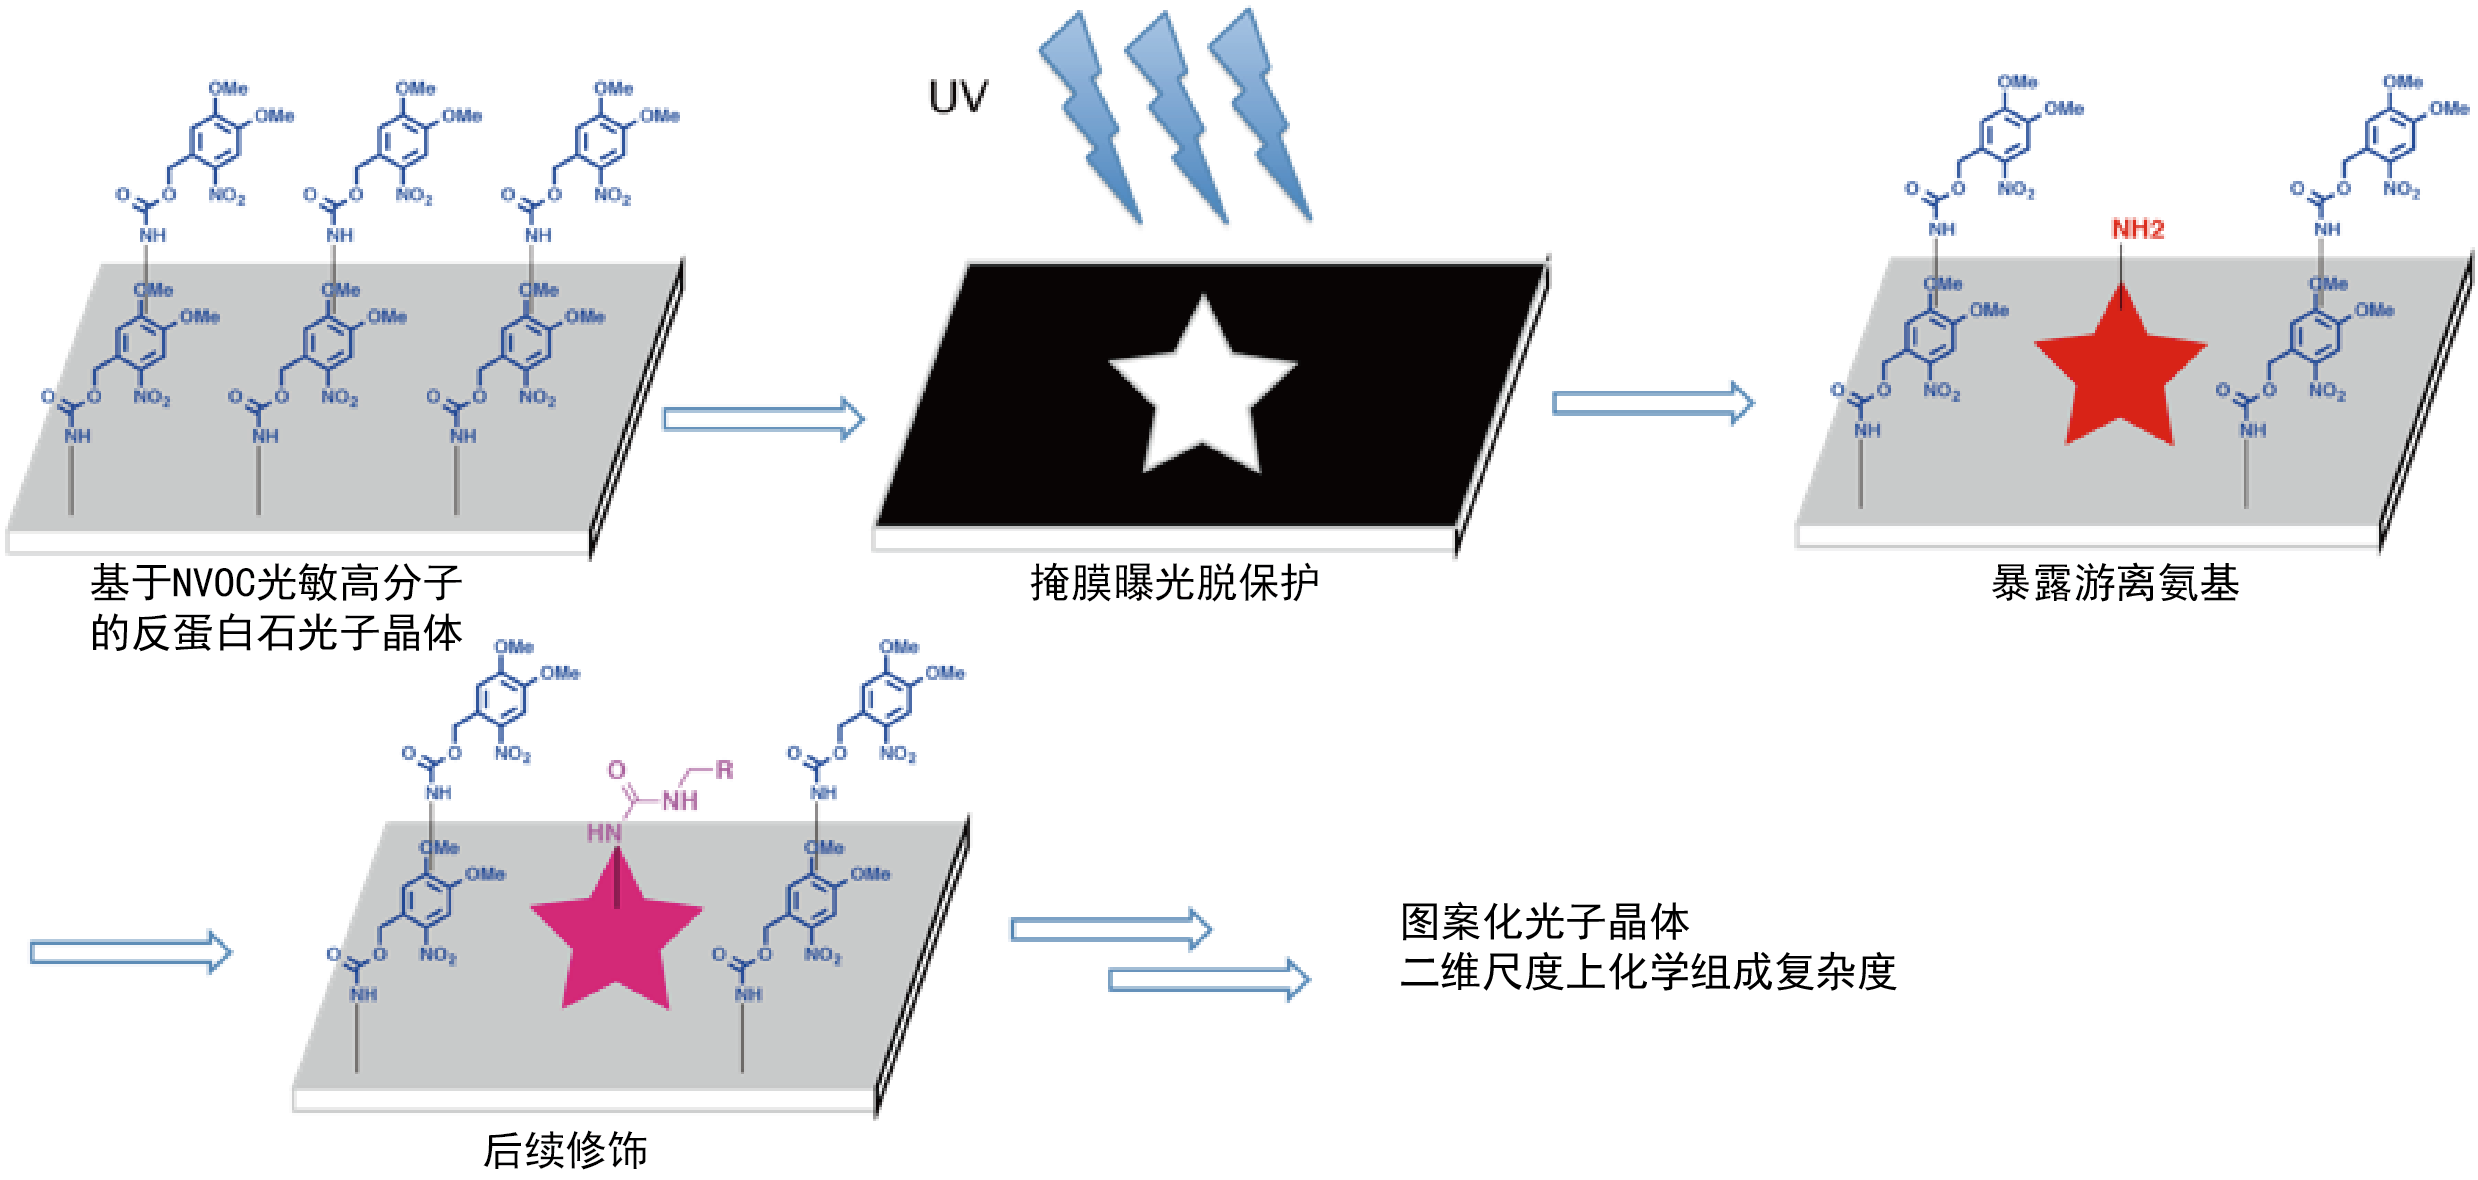
\includegraphics[width=\linewidth]{figures/ch4/scheme-2D-pattern.png}
  \caption{基于光敏高分子的光子晶体图案化方法原理示意图}
  \label{fig:photolabile-pattern-principle}
\end{figure}


本章中,我们将利用光敏高分子光子晶体在紫外光照条件下的可控脱保护-反应过程来对平面型的光子晶体进行图案化处理,赋予反蛋白石光子晶体二维尺度上化学复杂度。

\section{实验部分}
\label{sec:ch4-exp}

\subsection{实验材料与仪器}
本章中所使用的实验材料与仪器分别见表~\ref{tab:ch4-material}与~\ref{tab:ch4-instrument}。与前述章节重复的材料这里不再赘述。

\begin{table}[htbp]
  \centering
  \caption{本章所用实验材料}
  \label{tab:ch4-material}
    \begin{tabularx}{\linewidth}{XXXX}
      \toprule[1.5pt]
      {\heiti 药品名称} & {\heiti 纯度} & {\heiti 来源} & {\heiti 处理方法}\\
      \midrule[1pt]
      NaBH\text{$_4$} & 分析纯 & 国药集团化学试剂有限公司 & 直接使用\\
      2-硝基藜芦醛 & 分析纯 & 偶合试剂 & 直接使用\\
      1,3-丙二胺 & 分析纯 & 偶合试剂 & 直接使用\\
      二碳酸二叔丁酯(Boc\text{$_2$}O)& 分析纯 & 偶合试剂 & 直接使用\\
      N,N'-羰基二咪唑(CDI)& 分析纯 & 偶合试剂 & 直接使用\\
      N-羟基丁二酰亚胺(NHS)& 分析纯 & 国药集团化学试剂有限公司 & 直接使用\\
      二环己基碳二亚胺(DCC)& 分析纯 & 国药集团化学试剂有限公司 & 直接使用\\
      N,N-二甲基甘氨酸 & 98\% & Alfa Aesar & 直接使用\\
      三氟乙酸(TFA) & 98\% & Alfa Aesar & 直接使用\\
      \bottomrule[1.5pt]
    \end{tabularx}
\end{table}

\begin{table}[htbp]
  \centering
  \caption{本章所用仪器}
  \label{tab:ch4-instrument}
    \begin{tabularx}{\linewidth}{XXX}
      \toprule[1.5pt]
      {\heiti 仪器名称} & {\heiti 仪器规格} & {\heiti 厂家} \\
      \midrule[1pt]
      反射光纤光谱仪 & USB2000 & OceanOptics\\
      场发射扫描电子显微镜(SEM) & LEO-1503 & Bruker\\
      傅里叶变换红外光谱仪(FTIR)& PE 2000 & Perkin-Elmer\\
      核磁共振仪(NMR) & ECA 300 &JEOL\\
      电喷雾质谱仪(ESI) &Esquire-LC &Bruker\\
      接触角测定仪 & OCA 20 &Dataphysics\\
      透射式紫外可见光谱仪 & Lambda 35 &Perkin-Elmer\\
      台式紫外聚合仪 &自行搭建 &自行搭建\\
      \bottomrule[1.5pt]
    \end{tabularx}
\end{table}


\subsection{相关化合物的合成}
1. 含NVOC保护基的功能单体合成
含NVOC保护基的甲基丙烯酰胺单体的合成步骤见图~\ref{fig:NVOC-sync}。
\begin{figure}[htbp]
  \centering
  
\includegraphics[width=\linewidth]{figures/ch4/ch4-monomer-synth.png}
  \caption{含NVOC保护基的功能单体的合成步骤}
  \label{fig:NVOC-sync}
\end{figure}

对应的分子的合成步骤如下:

化合物3:将2.96 g (40.0 mmol,4 eqiv)1,3-丙二胺溶于100 mL干燥的CH\text{$_2$}Cl\text{$_2$}中,在冰浴条件下搅拌。同时,用恒压滴液漏斗将含2.18 g(10.0 mmol, 1eqiv)二碳酸二叔丁酯的CH\text{$_2$}Cl\text{$_2$}溶液(20 mL)缓慢滴加至烧瓶中,滴加过程在3 h中完成。随着二碳酸二叔丁酯的滴加,溶液中产生白色沉淀。滴加完毕后,抽滤除去白色不溶物,将有机相在饱和NaCl溶液中洗涤3次,并用CH\text{$_2$}Cl\text{$_2$}对水相反萃取一次。合并有机相,用Na\text{$_2$}SO\text{$_4$}干燥并旋蒸真空干燥。得到一透明粘稠液体(1.52 g,87\%)。
化合物3:叔丁基(3-氨丙基)氨基甲酸酯,\text{$^1$}H-NMR(300 MHz,CDCl\text{$_3$}): \text{$\delta$} 1.31-1.62 (11H, m, C(CH\text{$_3$})\text{$_3$} 以及C-CH\text{$_2$}-C), 2.73 (2H, t, NH\text{$_2$}CH\text{$_2$}), 3.15 (2H, t, CONH-CH\text{$_2$}),5.05 (2H, s, NH\text{$_2$})。ESI-MS: 175.2 [M+H]\text{$^+$}.

化合物4:将1.52 g (8.70 mmol, 1 eqiv)化合物3溶于20 mL CH\text{$_2$}Cl\text{$_2$}中,并与10 mL饱和NaHCO\text{$_3$}混合,在磁力搅拌器上预先搅拌。将1.26 g (12.0 mmol,1.4 eqiv)的甲基丙烯酰氯缓慢滴加到混合液中。
反应在常温下搅拌30 min。向反应液中加入50 mL CH\text{$_2$}Cl\text{$_2$}稀释,分离有机相并用饱和NaCl溶液洗涤2次。将有机相用Na\text{$_2$}SO\text{$_4$}干燥并旋蒸。粗产物以纯CH\text{$_2$}Cl\text{$_2$}进行逐层析分离。得到白色晶体(1.18g 59.4\%)。
化合物4:叔丁基(3-甲基丙烯酰氨丙基)氨基甲酸酯,\text{$^1$}H-NMR(300 MHz,CDCl\text{$_3$}): \text{$\delta$} 1.35 (s, 9H, C(CH\text{$_3$})\text{$_3$}), 1.64 (m, 2H, C-CH\text{$_2$}-C), 1.98 (s, 3H, CH\text{$_2$}-C=),3.15 (t, 2H, BocNH-CH\text{$_2$}), 3.36 (t, 3H, AcrylNH-CH\text{$_2$}), 5.39 (d, 1H, =CH), 5.79 (d, 1H, =CH)。ESI-MS: 243.6 [M+H]\text{$^+$}。

化合物5:将1.94 g (8.50 mmol)化合物4溶解于10 mL干燥的CH\text{$_2$}Cl\text{$_2$}中,在搅拌的同时向其中滴加2 mL TFA。随着反应进行,反应液中不断产生气泡。反应常温搅拌过夜。所得溶液在低温条件下旋蒸除去其中的溶剂及残留TFA。得到透明粘稠液体(0.884 g,81.2\%)。
化合物5:三氟乙酸氨丙基甲基丙烯酰胺,\text{$^1$}H-NMR(300 MHz,DMSO-d\text{$_6$}): \text{$\delta$}
1.64 (m, 2H, C-CH\text{$_2$}-C), 1.98 (s, 3H, CH\text{$_2$}-C=),3.36 (t, 3H, AcrylNH-CH\text{$_2$}), 5.39 (d, 1H, =CH), 5.79 (d, 1H, =CH), 7.66 (s, 3H, NH\text{$_3$}\text{$^+$})
。ESI-MS: 143.2 [M+H]\text{$^+$}。

化合物6:将4.22 g(20.0 mmol,2 eqiv)2-硝基藜芦醛分散在150 mL乙醇中并装入圆底烧瓶中。在搅拌过程中小心加入0.378 g (10.0 mmol, 1 eqiv)NaBH{$_4$}。将溶液温度升至回流,此时反应物逐渐在乙醇中溶解,溶液颜色加深。反应2 h后,将反应液冷却,旋蒸去除其中的乙醇,将粗产物用EA重新溶解,并在饱和NaCl溶液中洗涤2次。有机相干燥浓缩后用1:1 PE:EA柱层析分离。得到橙黄色固体(3.46 g,81.3\%)。
化合物6:2-硝基藜芦醇,\text{$^1$}H-NMR(300 MHz,CDCl\text{$_3$}): \text{$\delta$} 2.66 (s, 1H, OH), 4.00 (d, 6H, -OMe), 4.98 (s, 2H, CH\text{$_2$}), 7.17 (s, 1H, Ph-H), 7.69 (s, 1H, Ph-H)。ESI-MS: 226.1 [M+Na]\text{$^+$}。

化合物7:将1.82 g(8.54 mmol,1 eqiv)化合物6与1.38 g (8.54 mmol,1 eqiv)CDI溶于20 mL CH\text{$_2$}Cl\text{$_2$}中,常温搅拌12 h。将反应液用20 mLCH\text{$_2$}Cl\text{$_2$}稀释至100 mL,并用饱和NaCl溶液洗涤2次。收集有机相,用Na\text{$_2$}SO\text{$_4$}干燥,旋蒸得到淡黄色固体(2.45 g,93.7\%)。
化合物7:4,5-二甲氧基-2-硝基苯甲基-1-咪唑碳酸酯,\text{$^1$}H-NMR(300 MHz,CDCl\text{$_3$}): \text{$\delta$} 4.00 (d, 6H, -OMe), 4.98 (s, 2H, CH\text{$_2$}), 7.03 (d, 1H, =N-CH-CH), 7.17 (s, 1H, Ph-H), 7.40 (d, 1H, =N-CH-CH), 7.69 (s, 1H, Ph-H), 8.13 (d, 1H, N=CH-N)。ESI-MS: 308.8 [M+H]\text{$^+$}。


化合物8:将1.12 g (3.65 mmol, 1eqiv)化合物7与1.5 mL TEA溶于20 mL CH\text{$_2$}Cl\text{$_2$}中,在搅拌过程中,滴加入1.14 g (4.75 mmol, 1.3 eqiv)的化合物5。反应液避光常温搅拌过夜。待反应终止后,将反应液稀释至100 mL,并分别用1 M稀盐酸溶液、饱和NaCl溶液洗涤1次。将有机相干燥浓缩后用纯CH\text{$_2$}Cl\text{$_2$}展开剂进行柱层析提纯。得到白色至浅黄色絮状固体(0.909 g,65.4\%)。
化合物8:4,5-二甲氧基-2-硝基苯甲基(3-甲基丙烯酰氨丙基)氨基甲酸酯,\text{$^1$}H-NMR(300 MHz,CDCl\text{$_3$}): \text{$\delta$} 1.98 (s, 3H, CH\text{$_2$}-C=),3.36 (t, 3H, AcrylNH-CH\text{$_2$}), 4.00 (d, 6H, -OMe), 4.98 (s, 2H, CH\text{$_2$}), 5.39 (d, 1H, =CH), 5.79 (d, 1H, =CH), 6.59 (s, 1H, CONH), 7.17 (s, 1H, Ph-H), 7.69 (s, 1H, Ph-H)。ESI-MS: 404.2 [M+H]\text{$^+$}

2. 后修饰化合物合成
在脱保护后的后修饰中,涉及到活化羧基化合物的合成,其合成步骤如图~\ref{fig:postmod-sync}。
\begin{figure}[htbp]
  \centering
  
\includegraphics[width=0.75\linewidth]{figures/ch4/ch4-post-mod-synth.png}
  \caption{活化羧基的后修饰化合物合成步骤}
  \label{fig:postmod-sync}
\end{figure}

化合物9:将5.15 g(50.0 mmol,1 eqiv)N,N-二甲基甘氨酸、5.75 g(50.0 mmol,1 eqiv)N-羟基丁二酰亚胺与11.05 g(55.0 mmol,1.1 eqiv)DCC混合溶解于200 mL CH\text{$_2$}Cl\text{$_2$}中,在常温下搅拌反应20 h。反应生成的沉淀经过滤去除,滤液经浓缩后用1:2 PE:EA进行柱层析提纯,得到白色蜡状固体(2.35 g,23.2\%)。
化合物9:N,N-二甲基丙氨酸-(2,5-二氧代吡咯烷基)酯。text{$^1$}H-NMR(300 MHz,CDCl\text{$_3$}): \text{$\delta$} 2.42 (s, 6H, CH\text{$_3$}); 2.82 (s, 4H, CH\text{$_2$}CH\text{$_2$}); 3.52 (s, 2H, N-CH\text{$_2$})。ESI-MS:201.2 [M+H]\text{$^+$}。

\subsection{基于光敏高分子的反蛋白石光子晶体功能材料的制备}
这里基于光敏高分子的反蛋白石光子晶体的制备方法与\ref{subsec:evap-template}节中的方法类似,由于涉及后续的图案化操作,这里选用的光子晶体模板为利用LbL逐层堆积法生长的SiO\text{$_2$}模板,其他方面上略有不同:

1. 将NVOC保护的功能单体(化合物8) 50.0 mg (0.178 mmol)、30.2 mg (0.301 mmol)MMA、及 6.5 mg (0.033 mmol)EGDMA 溶于20 µL 热DMSO中,保持溶液温度在60 $^{\circ}$C上以防止NVOC功能单体析出,并加入5 \%质量分数的偶氮二异丁腈(AIBN)热引发剂。

2. 将SiO\text{$_2$}光子晶体模板(利用LbL逐层堆积法制备)与相同大小的PMMA基板制作三明治复合结构,预先对复合基板加热至50 $^{\circ}$C以上,并趁热用毛细作用将预聚液吸收入光子晶体缝隙中。将复合模板边缘用长尾夹固定牢固,用锡纸包裹放入80 $^{\circ}$C烘箱聚合24 h。

3. 将复合结构光子晶体从烘箱中取出冷却后,将光子晶体复合模板放入5 \%HF溶液中进行刻蚀约30 min,直到PMMA基板从玻璃片上脱落并呈现光子禁带颜色。

4. 将生长在PMMA基板上的反蛋白石光子晶体薄膜用乙醇-水洗涤去除HF及未聚合的部分单体,在氮气氛下干燥,即可用于后续的紫外脱保护及化学修饰。

5. 对反蛋白石光子晶体薄膜进行紫外脱保护时,将与光子晶体大小相当的图案掩膜与光子晶体薄膜贴合在一起,用胶条将其边缘轻微固定,光子晶体背面透明的部分用平整的锡箔纸包覆防止不必要的紫外光散射。将配合掩膜的光子晶体薄膜放置于200 mW/cm\text{$^2$}的360 nm紫外灯下以10 s为间隔进行照射脱保护。将脱保护后的光子晶体材料用乙醇-水洗涤以去除脱保护过程中产生的副产物。
所得的反蛋白石光子晶体即具有区域选择性的氨基成分。

6. 对上述脱保护后的光子晶体模板的后修饰如下:将用于后续修饰的化合物(异氰酸酯类、Suc活化羧酸或酰氯)配置为0.01-0.1 mol/L的DMF溶液。将经过脱保护处理的光子晶体表面滴加上述配制完的后修饰溶液,在暗处常温反应30 min - 2 h。之后小心地用滤纸吸残余的反应液,并用乙醇-水混合液小心洗涤2-3次,去除残留的反应物,并在氮气气氛下干燥。

\subsection{光敏高分子材料的表征}

1. 为了研究NVOC单体聚合的程度,我们采用与薄膜制备相同的配方,去除了交联剂EGDMA制备了含NVOC保护基的线性高分子。将50.0 mg (0.178 mmol)NVOC单体、30.2 mg (0.301 mmol)MMA及5 \%质量分数的AIBN溶于500 µLDMSO中,在氮气保护下与80 $^{\circ}$C油浴中搅拌反应24 h,溶液粘度显著增加。将聚合物溶液冷却后注入10 mL冷乙醚中,离心收集淡黄色沉淀,并用10 mL乙醚分散-离心洗涤2次,在真空干燥箱中干燥,得到琥珀色高分子60.5 mg (75.4 \%)。
将该高分子溶于CDCl\text{$_3$}中测定\text{$^1$}H-NMR。

2. 利用与光子晶体生长法相同的聚合物配比在有机玻璃片上生长一层含NVOC的光敏高分子,并切割为1 cm \text{$\times$} 4 cm的长条,以相同尺寸的空白PMMA基板作为本底,利用透射式UV-Vis光谱仪测定其在300 - 450 nm范围内的吸收光谱。含NVOC的光敏高分子薄膜分别以10 s为间隔在紫外光下照射脱保护,并测定对应的紫外-可见吸收。

\section{结果与讨论}
\subsection{基于NVOC光敏高分子的光子晶体表征}
本章中所使用的NVOC保护的甲基丙烯酸酯功能单体的聚合特性与之前所用的丙烯酸酯类单体有所不同。由于NVOC自身的吸收峰处于紫外至蓝紫光波段之间,用紫外光或可见光进行自由基聚合均会造成NVOC官能团的裂解。因此这种单体的聚合需要采用热引发的自由基聚合,采用AIBN作为自由基引发剂。
同时,由于含有硝基的芳香环结构能够吸收自由基,这种单体的聚合难度要高于其他甲基丙烯酸单体\cite{Schumers2009Are}。
因此,在聚合过程提高了自由基引发剂AIBN的含量,并延长了热聚合的时间以促进聚合物充分固化。
此外,由于单体含有酰胺及苯环等基团,在单纯的MMA中无法溶解,需要在加热的DMSO中溶解放能进行预聚液的灌注,而整个操作过程中需要保持光子晶体复合结构的温度,防止NVOC单体的析出。

在成功将含NVOC的甲基丙烯酸单体聚合的基础上,我们研究了聚合后的高分子在紫外光下脱保护的性能。首先,我们制备了线性的NVOC高分子,并研究了其NMR谱图。
\begin{figure}[htbp]
  \centering
  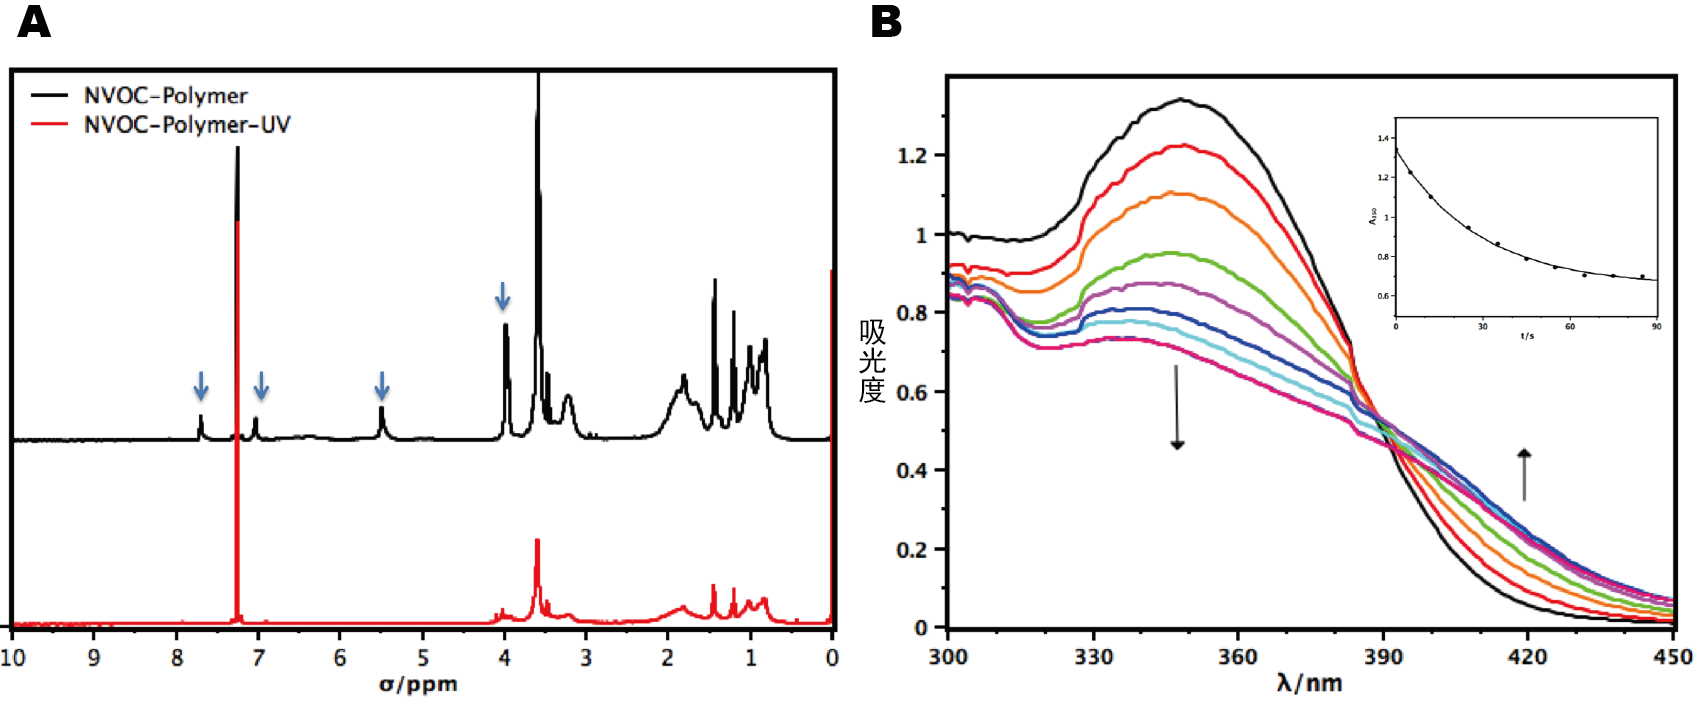
\includegraphics[width=\linewidth]{figures/ch4/NMR-IR.png}
  \caption{NVOC高分子的光反应表征。A. 线性高分子光照前后的NMR图谱对比;B. 高分子薄膜在光照过程中的紫外可见吸收变化。}
  \label{fig:NMR-IR}
\end{figure}

如图~\ref{fig:NMR-IR}A所示,聚合后的高分子中7.67、6.98 ppm处峰分别对应了NVOC中苯环上H的信号,5.41 ppm处为NVOC中的亚甲基H信号,而4.02 ppm处的峰对应了NVOC中的甲氧基H信号。
由NVOC的甲氧基H的积分与PMMA在3.53 ppm处的甲基H积分相比较,计算处NVOC单体在最终高分子中含量为17.6 \%。
这一含量低于实际投入的单体比,反应了NVOC单体较MMA而言聚合性能较差,只有部分参与了聚合。线性高分子中的NVOC含量比例能够一定程度上代表聚合物光子晶体中的含量比例。
经过360 nm紫外光照射60 s之后,原高分子的颜色由淡黄色转为深棕色,
这是由于NVOC在紫外光照射条件下产生的亚硝基副产物造成的\cite{Cui2011Polymer}。同时,其\text{$^1$}H-NMR中原来对应NVOC的所有特征峰均消失,说明了在60 s的光照时间之内脱保护已经完全。

同时,我们也利用了UV-Vis吸收光谱研究了含有交联剂的聚合物在UV照射下的脱保护过程(图~\ref{fig:NMR-IR}B)。
可以看出,随着UV照射时间的增加,聚合物在350 nm处的吸收显著下降,而在420 nm处的吸收有一定上升,在90 s的照射之后,聚合物的吸收趋于平稳。
其中,350 nm对应了NVOC的共轭吸收,而420 nm处的吸收来自于NVOC光解后的副产物。最终的吸收曲线并不为水平,这是由于含有功能高分子的基板与空白PMMA基板厚度不一致而造成的散射。
结合\text{$^1$}H-NMR与吸收光谱数据,可以说明含NVOC的光敏高分子在紫外光照射条件下的脱保护过程是快速而高效的。

\begin{figure}[htbp]
  \centering
  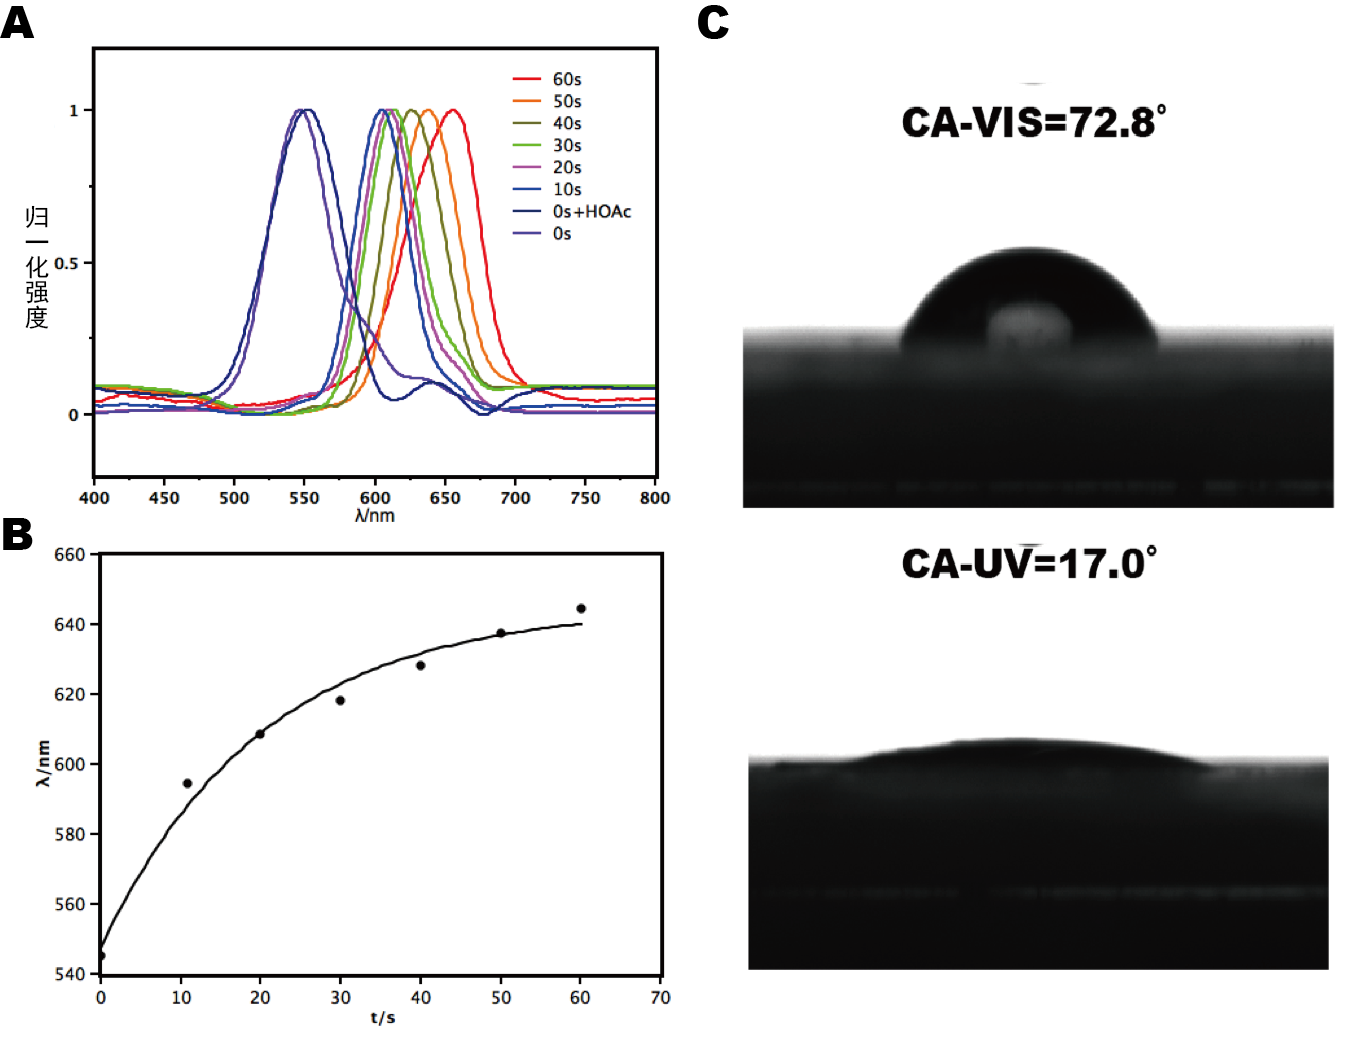
\includegraphics[width=0.85\linewidth]{figures/ch4/UV-Spectra.png}
  \caption{含有NVOC保护基团的光子晶体在光照前后的变化。A. 基于光敏高分子的光子晶体在光照前后的Bragg衍射峰变化;B. 对应A的时间-峰偏移曲线;C. 光照前后高分子的接触角变化}
  \label{fig:UV-spectra}
\end{figure}
此外,我们也对经过紫外光脱保护后光子晶体的化学环境变化进行了研究。如
	图~\ref{fig:UV-spectra}A、图~\ref{fig:UV-spectra}B
所示,经过紫外光照射之后,光子晶体的Bragg衍射峰位置发生了红移,这是由于在质子化条件下的氨基呈现强亲水性,而使光子晶体发生膨胀。
这也可以从平面高分子表面接触角在紫外照射前后的变化中得到证实(图~\ref{fig:UV-spectra}C)。
在未经过紫外光照射时,高分子表面接触角呈现相当疏水的72.8\text{$^\circ$}。
而经过UV照射1 min后,其接触角骤降至17.0\text{$^\circ$}。如此大的亲疏水性差异也是由脱保护后的氨基造成的。

\subsection{三维光子晶体的亲疏水梯度图案制备}

前述的材料表征证实了含NVOC的光敏高分子在光照条件下的脱保护过程是快速高效的,这里采用其可控氨基释放的性质结合高分子亲疏水性的变化来制备三维光子晶体上的亲疏水梯度图案。
这里我们设计了一种利用离散的点阵组成的光掩膜来制备梯度图案。如图~\ref{fig:photomask}所示,
这种光掩膜图案自左至右的透光部分呈现连续的变化。这里我们仅需通过单次UV照射来实现光子晶体上的梯度曝光。
\begin{figure}[htbp]
  \centering
  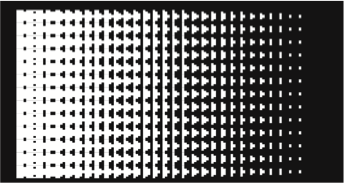
\includegraphics[width=0.45\linewidth]{figures/ch4/photomask.png}
  \caption{本节中使用的梯度光掩膜图案}
  \label{fig:photomask}
\end{figure}

通过这种方法制备的光子晶体亲疏水梯度图案如图~\ref{fig:photomask-gradient}所示,
\begin{figure}[htbp]
  \centering
  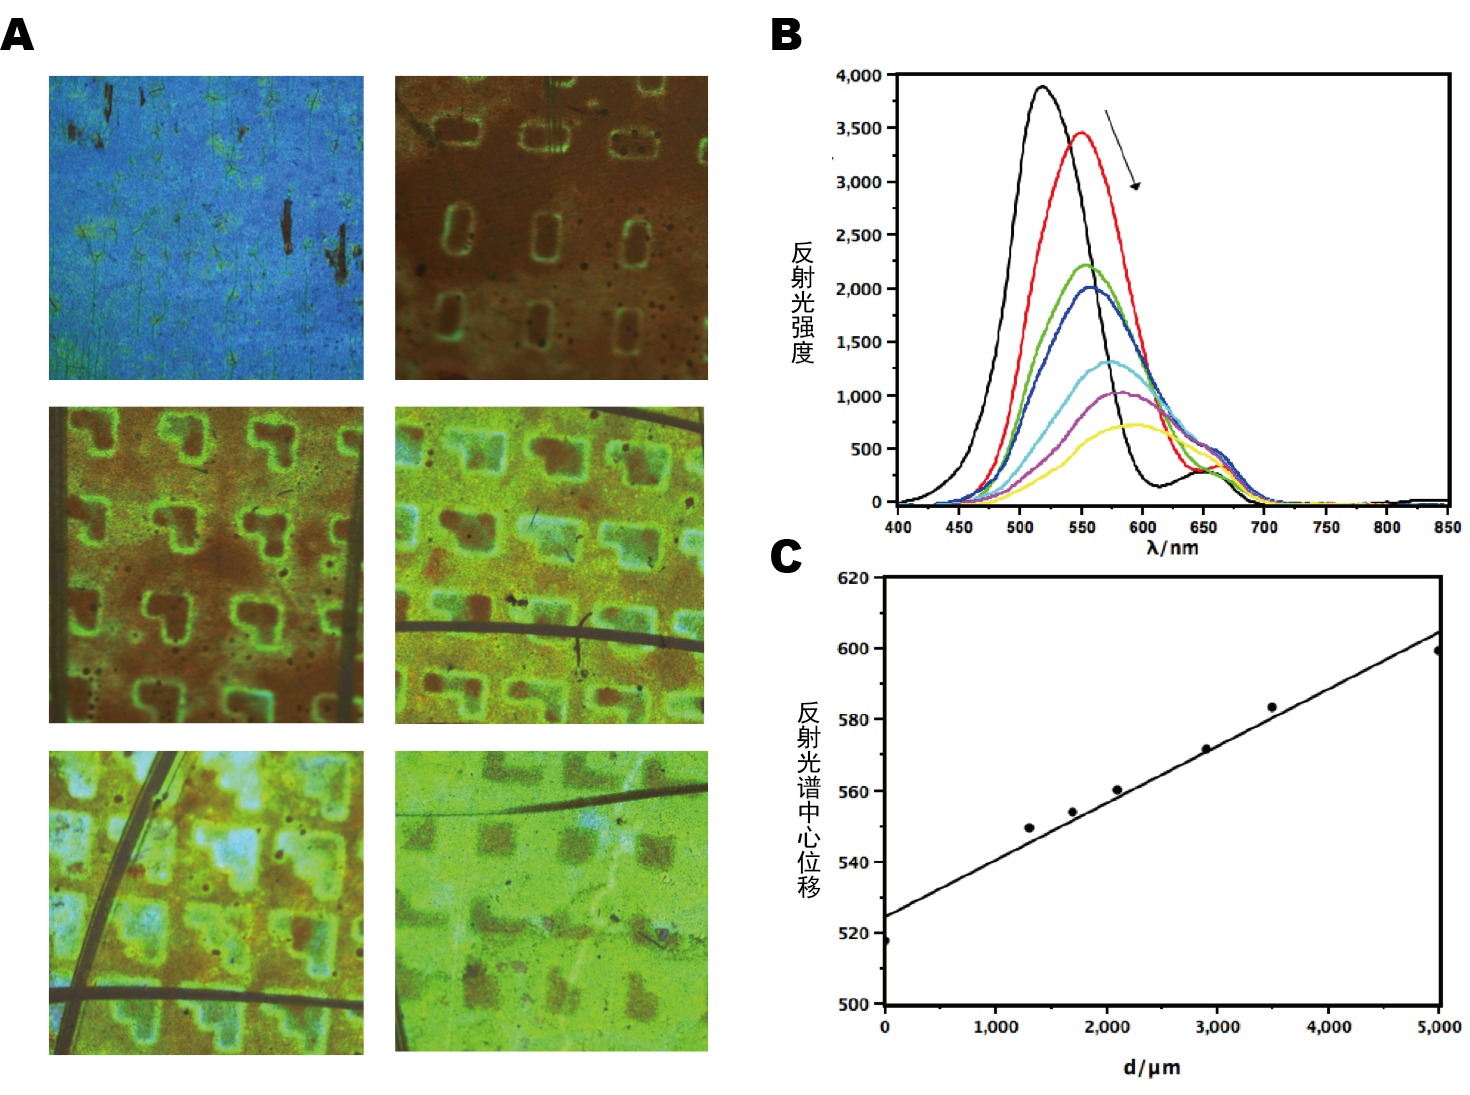
\includegraphics[width=0.85\linewidth]{figures/ch4/mask-gradient.png}
  \caption{利用掩膜法制备的光子晶体亲疏水图案。A. 亲疏水图各部位的显微光学照片;B. 光子晶体平均反射光谱随采样位置偏移的变化关系;C. 与B对应的反射光谱中心位移-物理位置之间的关系}
  \label{fig:photomask-gradient}
\end{figure}
在未经过照射的部分,光子晶体呈现蓝绿色的结构光性质,而随着曝光部分在水中“显影”后,具有结构化的图案便显现出来,随着曝光程度的升高,图案中绿色的未脱保护区域的组成逐渐减少,而暗红色的脱保护区域则逐渐增加(图~\ref{fig:photomask-gradient}A)。
这种特性也体现在其反射光谱上(图~\ref{fig:photomask-gradient}B、图~\ref{fig:photomask-gradient}C)。随着曝光面积的增加,其平均的Bragg衍射峰产生红移,且强度也由于长波段比例的增加而降低。其Bragg衍射峰位移与采样区域的相对位移呈现线性关系,说明这种亲疏水梯度的制备是成功的,且其亲疏水梯度能够直观地反映为光子晶体结构色的梯度变化。


本节中通过选择性光刻蚀的方法实现了光子晶体中的亲疏水梯度图案,
并将这种亲疏水梯度在光子晶体禁带结构上反应出来。
这种亲疏水梯度可以作为驱动力来诱导溶剂在反蛋白石结构内部的通透\cite{Burgess2012Wetting}。同时,线性变化的光子晶体禁带结构也可以用于光子晶体光谱仪等应用\cite{Ding2014Responsive}。

\subsection{三维光子晶体的动态图案制备}

上一节中我们利用了光反应后释放的游离氨基产生的亲疏水性差异制备了具有亲疏水梯度图案的光子晶体。这里我们将进一步利用脱保护-修饰的方法来制备具有动态响应性的光子晶体图案。
这里我们在光子晶体中实现两种具有不同化学组成的图案。其一由异氰酸丙酯对氨基进行修饰,另一则由活化的N,N-二甲基丙氨酸进行修饰。
其中,异异氰酸酯修饰的区域处于化学惰性,不随pH产生响应;而相反,修饰上三级胺基团的部分则呈现pH相关的质子化响应。
同时,由于三级胺的弱碱性,这种质子化过程在CO\text{$_2$}/N\text{$_2$}的循环下是可逆的(图~\ref{fig:reversible-protonation})\cite{Han2012General}。
\begin{figure}[htbp]
  \centering
  
\includegraphics[width=0.5\linewidth]{figures/ch4/tertial-amine.png}
  \caption{三级胺化合物在CO\text{$_2$}/N\text{$_2$}循环下的可逆质子化过程}
  \label{fig:reversible-protonation}
\end{figure}

因此我们期望通过赋予光子晶体不同的化学组成,实现动态调控的光子晶体图案。如图~\ref{fig:realsample}所示,通过上述方法制备的图案化光子晶体具有差异性的两部分图案,同时,由于光子晶体自身的特性,这种图案需要在反射条件下才能明显观察出来。
其中,内部的“THU”字样有由异氰酸酯进行修饰,而外侧的背景则修饰上三级胺组分。由于两处组分的折射率存在差别,因此显现处不同的结构色。
\begin{figure}[htbp]
  \centering
  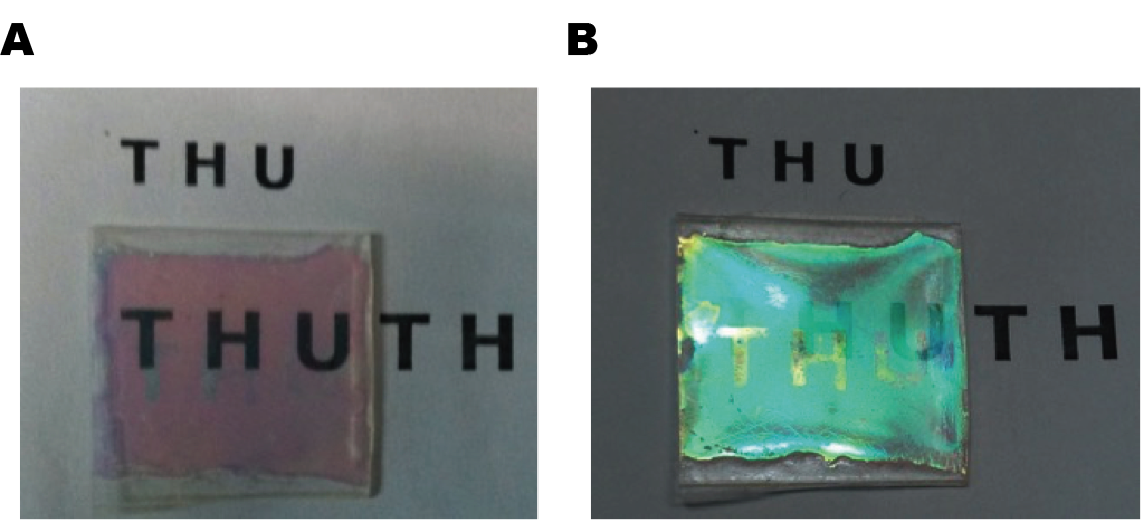
\includegraphics[width=0.8\linewidth]{figures/ch4/realsample.png}
  \caption{具有结构色图案的光子晶体实物照片。A. 透射视角;B. 反射视角}
  \label{fig:realsample}
\end{figure}


如图~\ref{fig:dynamic_pattern}所示,当这种图案化的光子晶体材料与CO\text{$_2$}在水相中反应时,外部三级胺组分被质子化,因此其光子禁带产生红移,内部字样图案由于其化学惰性组分,光子禁带几乎没有偏移。在与CO\text{$_2$}反应前后,两者的Bragg衍射峰差异由原来的122 nm 减少至 35 nm,使得内外部图案的差异变小,原始的字母图案的的观察较为困难。而对质子化的高分子进行N\text{$_2$}鼓泡后,外层光子晶体背景的图案去质子化而回复原始的图案。
\begin{figure}[htbp]
  \centering
  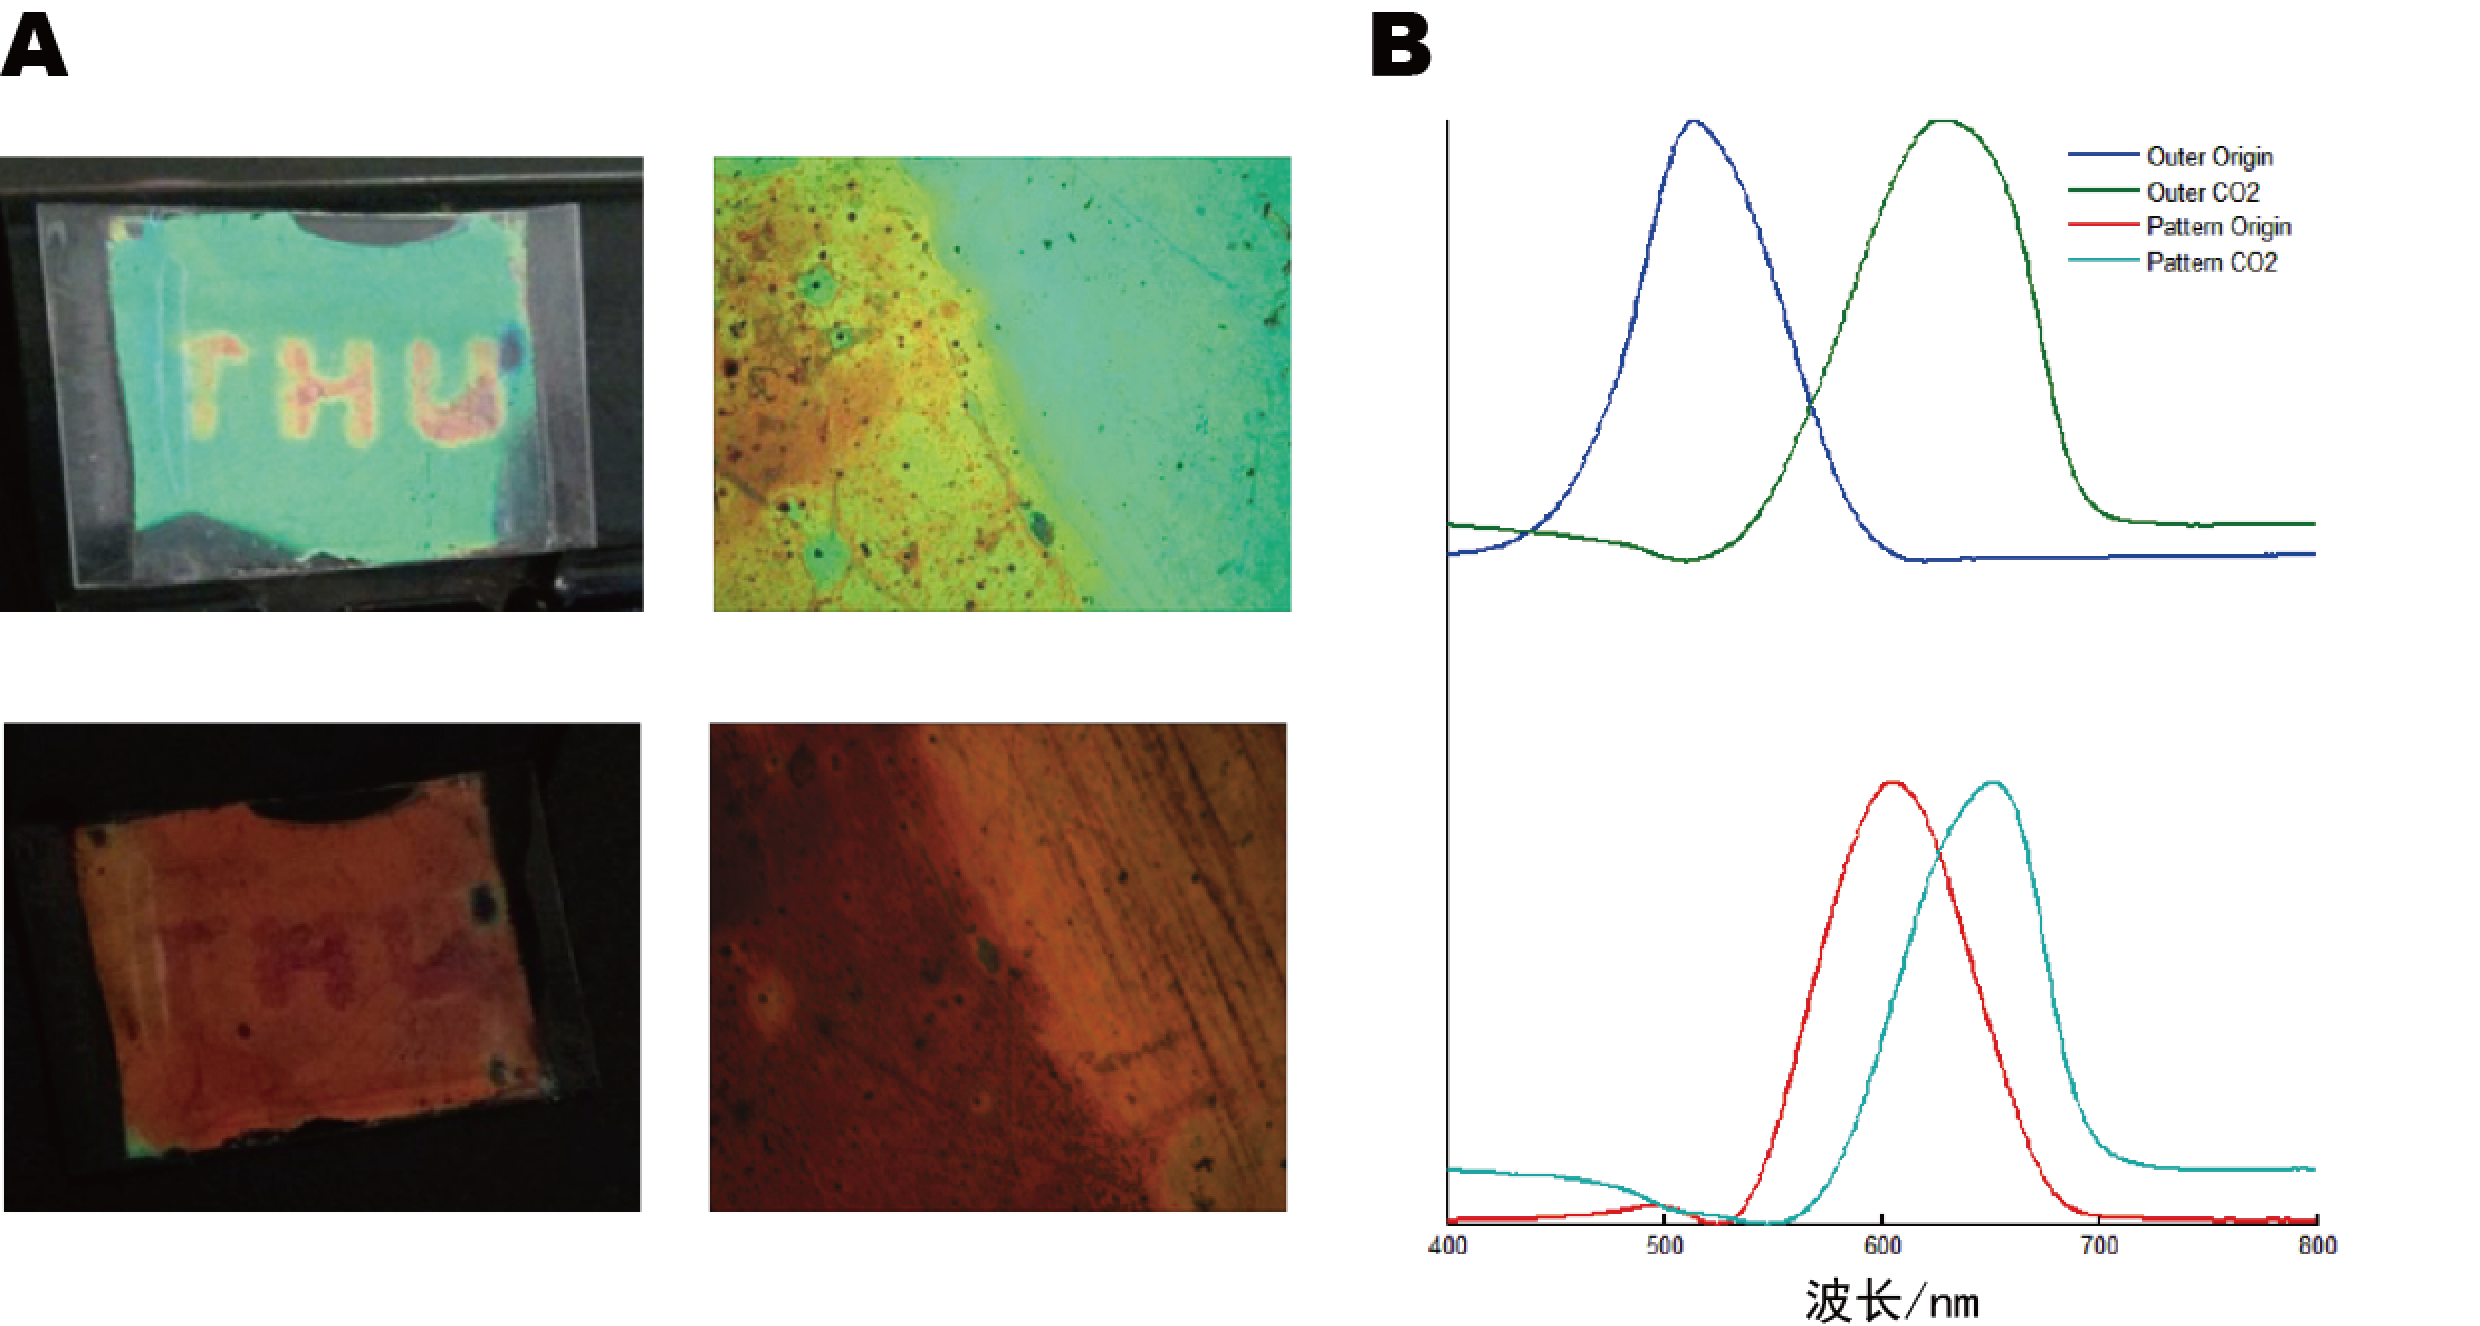
\includegraphics[width=\linewidth]{figures/ch4/dynamic-pattern.png}
  \caption{光子晶体图案在CO\text{$_2$}/N\text{$_2$}循环下的动态调节。A 非质子化(上)与质子化(下)的光子晶体图案光学照片及其图案边界显微照片;B. 动态调节的光子晶体图案的Bragg衍射峰在质子化与非质子化情况下的变化}
  \label{fig:dynamic_pattern}
\end{figure}


此外,我们就这种光子晶体材料的动态响应特性进行了表征。如图~\ref{fig:CO2-saturation}所示,尽管CO\text{$_2$}与高分子的反应平衡需要20 min以上,但在最初的5 min中CO\text{$_2$}造成的高分子质子化就对光子晶体禁带的偏移贡献了约75\%,说明这种反应是快速高效的。同时,我们对图案的动态调控进行了循环测试,在5次循环过程中,外部图案的Bragg衍射峰能够可逆地变化,说明了含有三级胺的光子晶体图案在CO\text{$_2$}/N\text{$_2$}循环处理下的可逆性。
\begin{figure}[htbp]
  \centering
  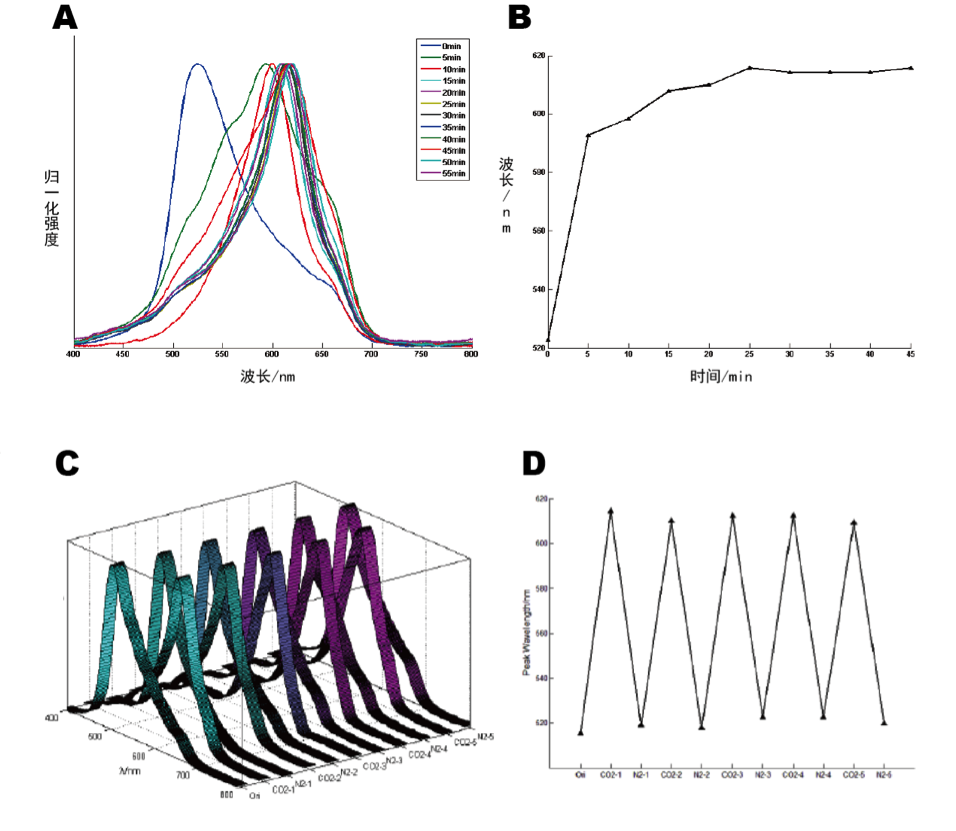
\includegraphics[width=0.85\linewidth]{figures/ch4/CO2-saturation.png}
  \caption{光子晶体动态图案的性能测试。A. 反射光谱随CO\text{$_2$}反应时间的变化;B. 与A.对应的光子晶体Bragg衍射峰位置与CO\text{$_2$}反应时间的变化曲线;C. 光子晶体反射光谱随CO\text{$_2$}-N\text{$_2$}循环的变化;D. 与C相对的循环曲线。}
  \label{fig:CO2-saturation}
\end{figure}

本节中利用光脱保护-修饰的方法实现了平面型光子晶体上的动态图案化。这种基于CO\text{$_2$}/N\text{$_2$}可逆响应的图案化光子晶体材料在CO\text{$_2$}的传感以及防伪材料方面具有潜在应用前景,能够提供一种直观的CO\text{$_2$}指示方法。同时,由于光敏高分子脱保护产生的氨基能够实现非常多样的后修饰目的,可以预期利用这种基于光敏高分子的光子晶体作为平台,发展一系列具有图案化及复杂化学组成的光子晶体材料。


\section{本章小结}

本章中基于光敏高分子实现了平面反蛋白石光子晶体的图案化与复杂化学组成修饰等应用。利用NVOC保护基在紫外光照下可控脱保护与修饰的特性,发展了一种在平面型反蛋白石光子晶体材料上图案化的方法,这种光子晶体修饰方法操作简便,内部结构稳定,且通过反应后修饰赋予了光子晶体很大的拓展性。基于这种平面型光子晶体图案化的方法,分别展示了两种拓展应用:基于选择性光反应-修饰法制备了光子晶体亲疏水梯度图案,以及基于选择性光反应-修饰法制备动态调节的图案化光子晶体。
基于这种脱保护-修饰的图案化光子晶体平台,可以进一步发展具有复杂化学组成、光学特性的功能材料及防伪材料。